\section{Patterns 6 - Redegør for følgende concurrency mønstre}

\subsection{Fokuspunkter}

\begin{itemize}
	\item Futures.
	\item Pipelines.
\end{itemize}

\subsection{Future}
Vi starter ud med lidt om \textbf{dependancies}:

Afhængigheder er et problem for parallelisering.
Vi sorterer det der kan paralleliseres og gør det!

\begin{figure}[h]
\centering
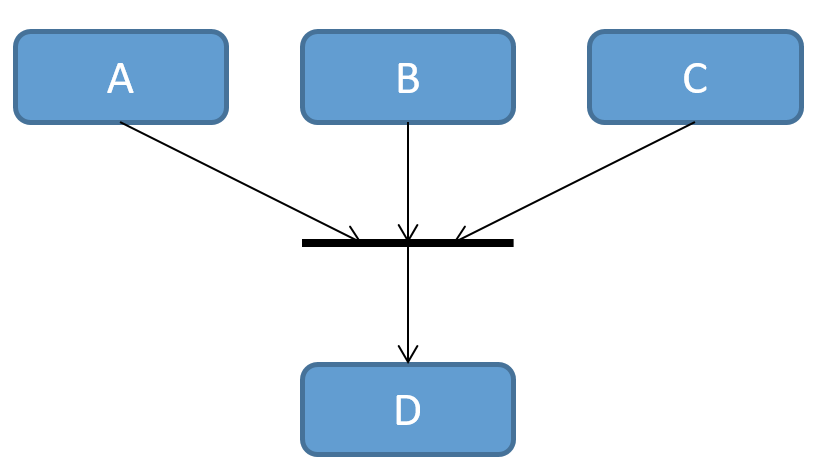
\includegraphics[width=0.5\linewidth]{figs/pipeFut/dependancies.PNG}
\caption{Node D skal køres før A, B og C kan køres parallelt}
\label{fig:dependancies}
\end{figure}

En future kan betegnes som en stand-in for en værdi der som udgangspunkt er utilgængelig, men som bliver tilgængelig på et senere tidspunkt.
Altså bruges futures når vi ønsker at parallelisere kode der har data dependancies.

\begin{figure}[h]
	\centering
	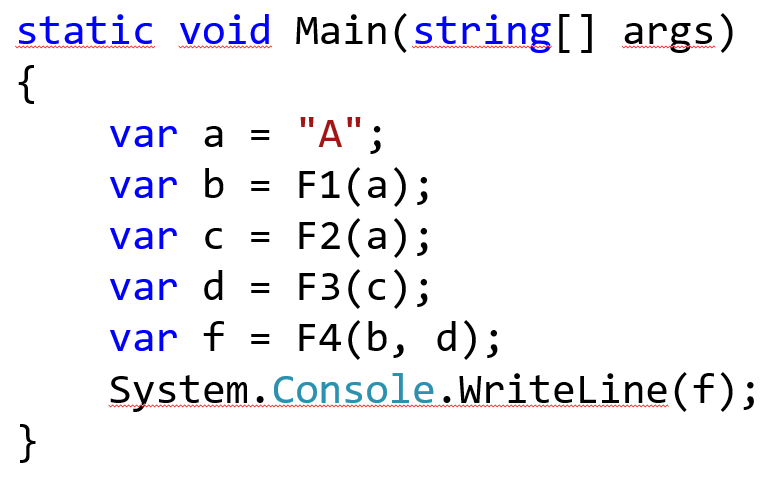
\includegraphics[width=0.5\linewidth]{figs/pipeFut/parallelThis.PNG}
	\caption{Data dependancies}
	\label{fig:Datadependancies}
\end{figure}

Vi laver en dependancy til en future! Altså et løfte om at den kommer!

\begin{figure}[H]
	\centering
	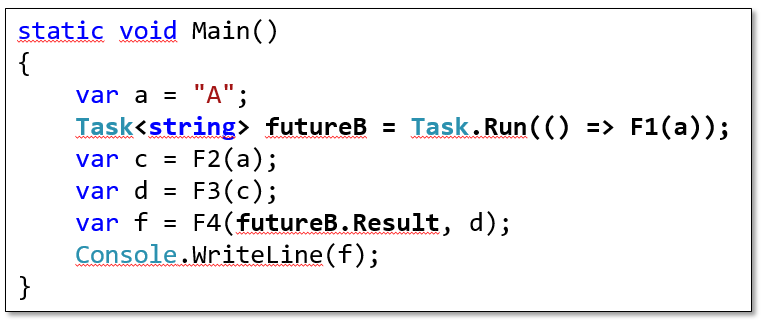
\includegraphics[width=0.6\linewidth]{figs/pipeFut/futureB}
	\caption{Brug af Futures}
	\label{fig:FutureEx}
\end{figure}

\subsection{Pipelines}
\begin{itemize}
	\item Pipeline mønstret paralleliserer processeringen af en input sekvens.
	\item Pipeline mønstret består af en serie af producer/consumere.
	\item Opdeler processering i paralelliserbare stadier
	\begin{itemize}
		\item Output af stage i er indput i stage i + 1:
		\item Andre stadier er uafhængige.
	\end{itemize}
\end{itemize}


